\documentclass[addpoints,12pt,twoside]{exam} %answers 
\usepackage[paper=a4paper,left=15mm,right=15mm,top=25mm,bottom=25mm]{geometry}
\usepackage{graphicx}
%\usepackage[dvips]{graphicx}
\usepackage{floatflt,epsfig} 
\usepackage{ngerman}
\usepackage{german}
\usepackage[utf8]{inputenc}
\usepackage{amssymb, amsmath}
\usepackage[gate,ic,optics]{circ}
\usepackage{hyperref}

\usepackage{tikz,pgfplots}

\usepackage{graphicx}
%\usepackage{geometry}
\usepackage{calc}


\usepackage{qrcode} 
\usepackage{wrapfig}
\usepackage{gensymb}
\usepackage{siunitx}

\usepackage{color}
\definecolor{GridColor}{gray}{0.8}
\definecolor{SolutionBoxColor}{gray}{0.8}
\definecolor{SolutionColor}{rgb}{0.8,0.9,1}

\colorgrids
\colorsolutionboxes 

%%MACROS 
\newcommand{\tdate}{7. Mai 2021}
\newcommand{\myqr}{\qrcode[hyperlink, height = 1cm]{www.github.com/shahrrks}}
\newcommand\gauss[2]{1/(#2*sqrt(2*pi))*exp(-((x-#1)^2)/(2*#2^2))} % Gauss function, parameters mu and sigma
%%
\newcommand{\drawgraph}{ 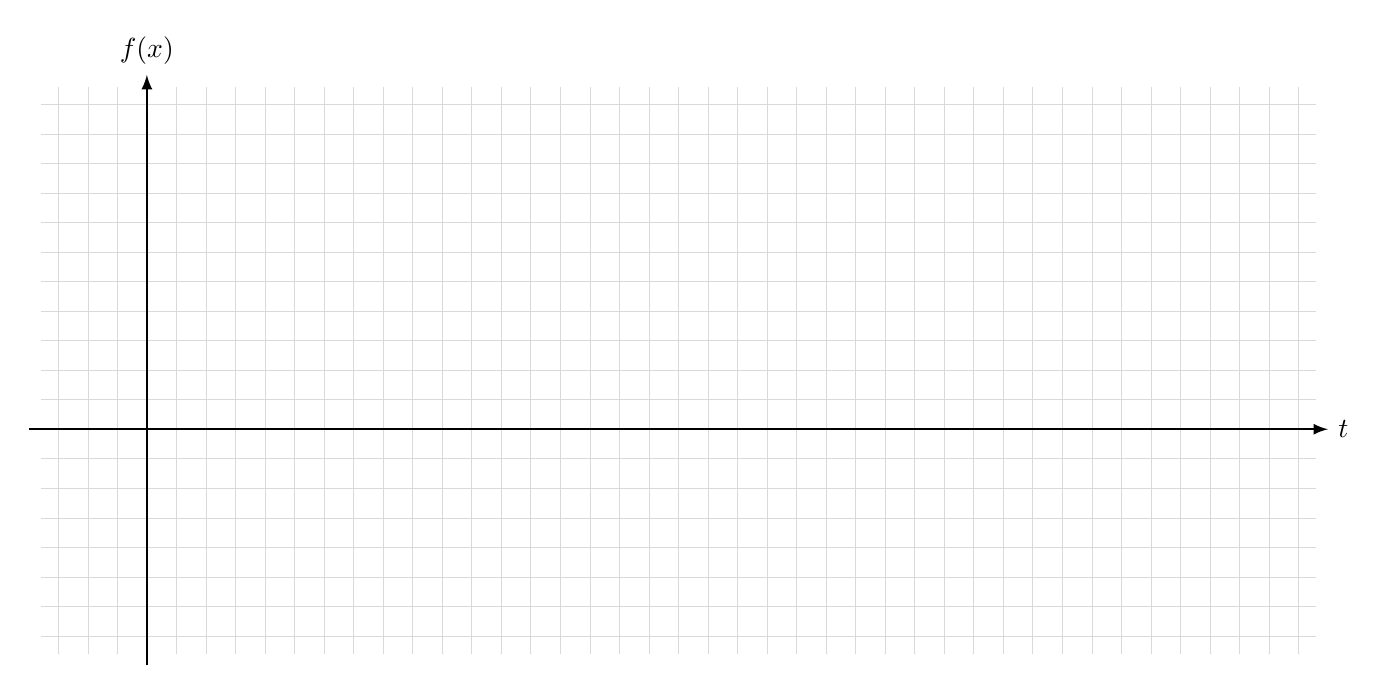
\begin{tikzpicture}[scale = 1.5]
	\draw[step=.25cm,gray!30,very thin] (-3.9,-1.9) grid (6.9,2.9);
	\draw[style = thick,black, -latex] (-4,0) -- (7,0) node[right] {\( t  \)};
	\draw[style = thick,black, -latex](-3,-2) -- (-3,3) node[above]{\( f(x)  \)};
\end{tikzpicture}}
%%

\sisetup{
locale = DE ,
per-mode = symbol
}

\pagestyle{headandfoot}

\headrule
\footrule
\firstpageheader{ETIT-4}{\bfseries\Large {Übungsblatt 5}}{\tdate}
\runningheader{ETIT-4}
{Übungsblatt - 5}
{\tdate}
\firstpagefooter{ETIT-4}{Seite \thepage\ von \numpages}{\myqr}
\runningfooter{ETIT-4}{Seite \thepage\ von \numpages}{Shah Rrks}

\boxedpoints
%\pointpoints{Punkt}{Punkte}
\pointsinmargin
\marginpointname{\%}


\begin{document}
%\setcounter{section}{1} %current page -1
\section*{Sys1}
\begin{questions}
\question[5]
\[ x(t) =
\begin{cases}
0 & falls \; t < 0 \\
t & falls \; 0 \leq t \leq 2 \\
2 \exp^{-(t-2)} & sonst

\end{cases}  \] 

\drawgraph

\question[5]
\[ x(t) = \varepsilon (t) \cdot t^2 \cdot \sin(8\pi t)  \]

\drawgraph

\pagebreak


\begin{figure}[h]
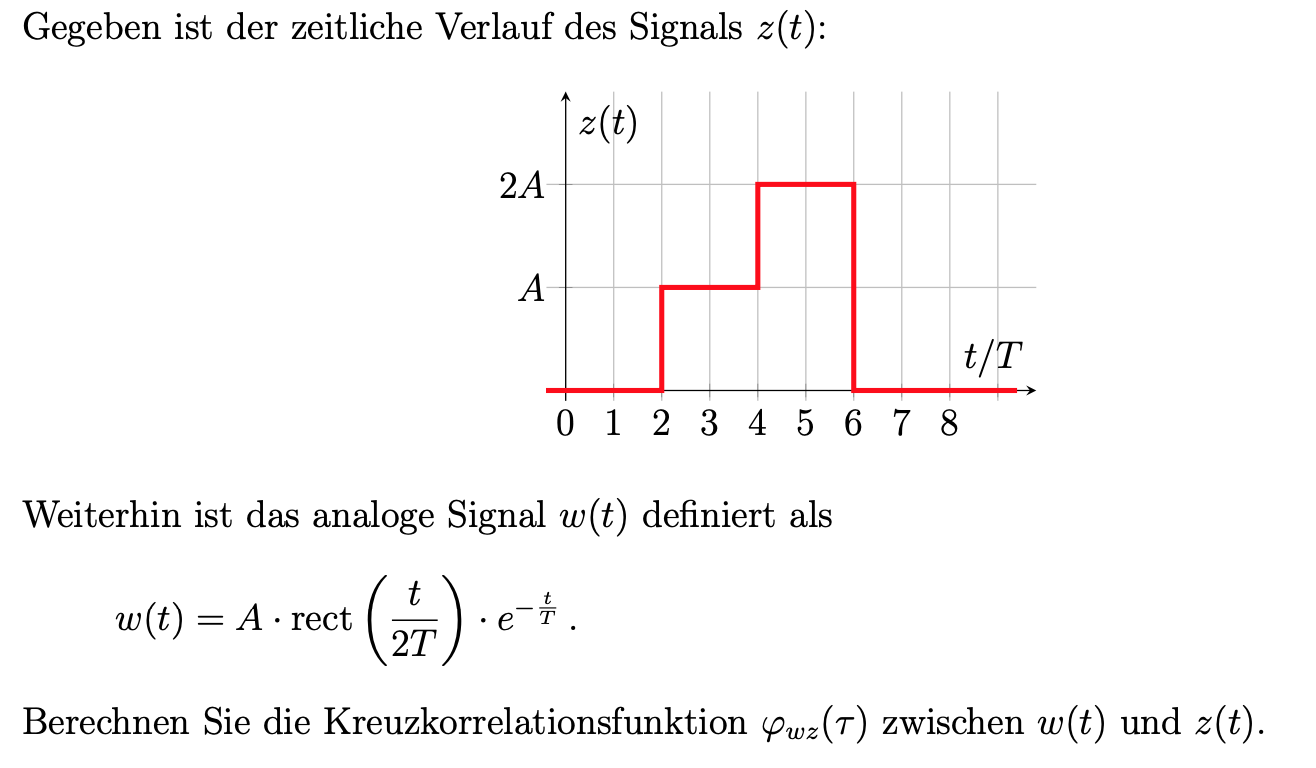
\includegraphics[width=0.8\textwidth]{auf3}
\end{figure}
\pagebreak
\section*{ET-2}
\begin{figure}[h]
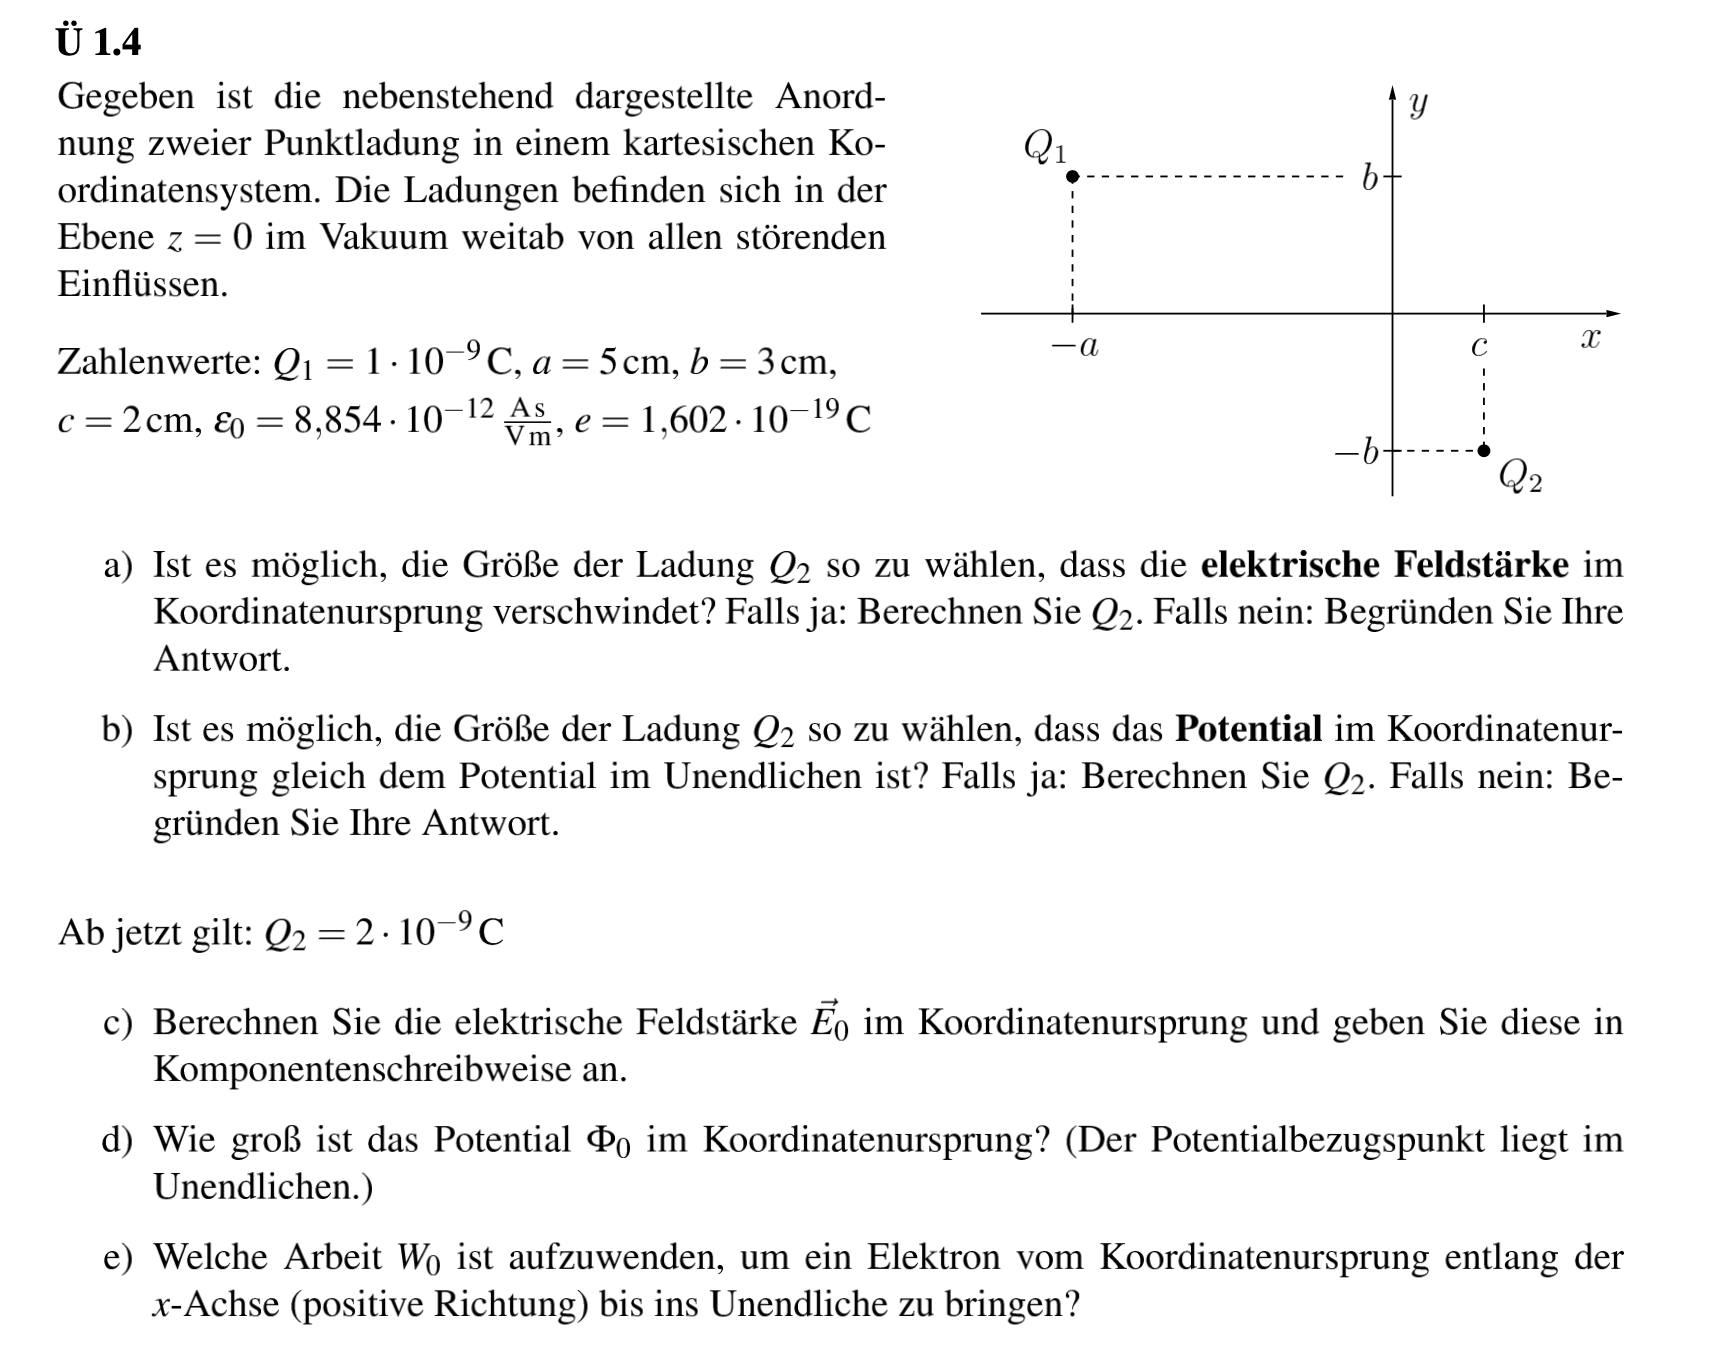
\includegraphics[width=0.96\textwidth]{auf4.png}
\end{figure}
\end{questions} 


\section{This is a Section}
\subsection{This is a subsection}
\subsection{This is another subsection}
\subsection{another Subsection}
\subsubsection{This is sub subsection}
\subsubsection{This is sub sub section}
\end{document}